\documentclass[conference]{IEEEtran}
\IEEEoverridecommandlockouts

% --- PACOTES RECOMENDADOS ---
\usepackage[utf8]{inputenc}
\usepackage[brazilian]{babel}
\usepackage{amsmath,amssymb,amsfonts}
\usepackage{graphicx}
\usepackage{textcomp}
\usepackage{xcolor}
\usepackage{booktabs}
\usepackage{multirow}
\usepackage{url}
\usepackage{cite}
\usepackage{float}
\raggedbottom 

\begin{document}

% --- TÍTULO E AUTORES (PADRÃO IFBA / ADS) ---
\title{Modelagem Preditiva de Decisões Judiciais nas Varas de Relações de Consumo da Comarca de Salvador com Aprendizado de Máquina}

\author{
    \IEEEauthorblockN{Vinícius Matos dos Santos}
    \IEEEauthorblockA{\textit{Curso de Análise e Desenvolvimento de Sistemas} \\
    \textit{Instituto Federal da Bahia (IFBA)}\\
    Salvador, Bahia, Brasil \\
    viniciusmatoslyon@gmail.com}
    \and
    \IEEEauthorblockN{Pablo Vieira Florentino}
    \IEEEauthorblockA{\textit{Departamento de Computação} \\
    \textit{Instituto Federal da Bahia (IFBA)}\\
    Salvador, Bahia, Brasil \\
    pablovf@ifba.edu.br}
}

\maketitle

% --- RESUMO E KEYWORDS (COMENTADOS CONFORME DIRETRIZ DO ALUNO) ---
% \begin{abstract}
% \end{abstract}
% \begin{IEEEkeywords}
% \end{IEEEkeywords}

% --- I. INTRODUÇÃO ---
\section{Introdução}
\IEEEPARstart{O}{ecossistema} processual brasileiro gerencia um alto volume de litígios de massa, gerando bases de dados estruturadas gigantescas e padronizadas pelo Conselho Nacional de Justiça (CNJ) por meio da plataforma DataJud \cite{cnj_datajud}. Com o recente movimento de modernização tecnológica do Judiciário, a adoção de sistemas baseados em inteligência artificial tornou-se uma pauta prioritária. Contudo, nesse cenário complexo, a imprevisibilidade das decisões e a altíssima demanda de processos judiciais ainda dificultam a gestão e a análise estratégica de riscos, especialmente no congestionado âmbito do Direito do Consumidor \cite{lage2022, bertalan2020}.

Para lidar com esse grande volume de dados, a jurimetria, estruturada no contexto brasileiro por Zabala e Silveira \cite{zabala2014} como a aplicação de métodos quantitativos e estatísticos ao Direito, surge como uma abordagem objetiva para analisar a jurisprudência e tornar a aplicação da lei mais previsível. A capacidade de prever ou classificar eventos jurídicos por meio do aprendizado de máquina tem se mostrado fundamental tanto para a gestão de litígios por escritórios de advocacia quanto para o mapeamento de gargalos processuais pelos próprios tribunais \cite{aletras2016, katz2017}. Embora a jurimetria forneça o alicerce teórico para a compreensão empírica dos dados, o presente trabalho aborda este cenário estritamente sob a ótica da Ciência da Computação. Nesse sentido, o escopo delimita-se à tarefa de predição supervisionada, diferenciando-se da modelagem causal tradicional para focar no desafio da modelagem preditiva e na avaliação comparativa de algoritmos sob rigor metodológico \cite{izbicki2020}.

Entretanto, a modelagem de desfechos judiciais enfrenta o desafio da alta aleatoriedade inerente aos dados. Conforme postulado pelo modelo microeconômico de seleção de litígios de Priest e Klein \cite{priest1984, trecenti2021}, demandas judiciais cujo desfecho probatório é evidente tendem a ser resolvidas por acordos extrajudiciais ou conciliações pré-processuais. Isso deixa para a fase de julgamento de mérito apenas as disputas limítrofes, nas quais a probabilidade de vitória de ambas as partes é balanceada e naturalmente incerta. Dessa forma, a integração de algoritmos de aprendizado de máquina na predição de decisões exige não apenas alto poder de discriminação preditiva, mas robusta explicabilidade para lidar com esse ruído intrínseco aos litígios submetidos à sentença definitiva.

Diante deste cenário, o presente artigo investiga a aplicação de diferentes famílias de algoritmos de aprendizado de máquina para a classificação de desfechos processuais das Varas de Relações de Consumo da Comarca de Salvador, englobando desde modelos lineares paramétricos clássicos até arquiteturas complexas de \textit{ensemble}. O intuito é avaliar rigorosamente o ganho preditivo de cada abordagem frente à sua interpretabilidade, estabelecendo um referencial metodológico seguro para a aplicação de algoritmos preditivos no Judiciário baiano.

\subsection{Problema de Pesquisa}
Qual é o desempenho de diferentes algoritmos de aprendizado de máquina, alimentados por metadados processuais e pelas Tabelas Processuais Unificadas (TPU), na classificação de sentenças de mérito das Varas de Relações de Consumo da Comarca de Salvador? Complementarmente, existe um ganho preditivo que justifique o uso de algoritmos complexos não-paramétricos em detrimento de modelos lineares interpretáveis sob as mesmas condições e dimensionalidade de variáveis? E de que forma a extração de coeficientes permite mensurar a força associativa do órgão julgador e da matéria sobre essas decisões?

\subsection{Objetivo Geral}
Desenvolver e comparar o desempenho de diferentes algoritmos de classificação na predição do desfecho de processos de Direito do Consumidor em primeira instância. Busca-se avaliar, sob a ótica do controle de complexidade e do balanço viés-variância, se modelos não-paramétricos mais complexos superam estatisticamente modelos \textit{baseline} interpretáveis, sob as mesmas condições e dimensionalidade de variáveis extraídas da API pública do DataJud (CNJ).

\subsection{Objetivos Específicos}
Para atingir o objetivo geral deste trabalho, realizou-se a extração e higienização da base empírica estruturada da API pública do DataJud, estabelecendo uma partição temporal estrita (\textit{out-of-time}) entre as safras de treinamento (2020 a 2023) e teste cego (2024), visando prevenir o vazamento de dados (\textit{data leakage}) \cite{hyndman2021}.

Em seguida, construiu-se uma matriz dimensionalmente simétrica de 74 covariáveis, aplicando codificação bayesiana \textit{out-of-fold} para atributos de alta cardinalidade do órgão julgador e assuntos da TPU \cite{miccibarreca2001, izbicki2020}, integrada à binarização de variáveis temporais cíclicas e matérias jurídicas recorrentes de consumo.

Para essa representação, avaliaram-se os algoritmos supervisionados sob particionamento temporal expansivo (\textit{TimeSeriesSplit}), calibrando limiares ótimos de decisão (\textit{threshold tuning}) a partir das curvas de precisão e revocação \cite{izbicki2020}.

Por fim, compararam-se três abordagens de modelagem supervisionada: (i) a Regressão Logística regularizada com penalização \textit{ElasticNet} como linha de base (\textit{baseline}) interpretável \cite{zou2005, izbicki2020}; (ii) o Fluxo Alternativo 1 (FA1), empregando o algoritmo \textit{Random Forest} \cite{breiman2001} com redução de variância por \textit{bagging}; e (iii) o Fluxo Alternativo 2 (FA2), utilizando o algoritmo \textit{XGBoost} \cite{chen2016} via aprendizado sequencial aditivo (\textit{gradient boosting}). A comparação considerou o desempenho computacional e preditivo por meio das métricas de ROC-AUC, Acurácia, Precisão, Sensibilidade (\textit{Recall}) e \textit{F1-score}, complementadas por intervalos de confiança a 95\% via \textit{bootstrapping}, de modo a fundamentar a seleção do modelo sob o Princípio da Parcimônia (Navalha de Ockham)~\cite{izbicki2020}.

% --- II. RECURSOS COMPUTACIONAIS ---
\section{Recursos Computacionais}
Os experimentos foram executados em um computador equipado com processador Intel Core i5-12500H com arquitetura híbrida de 12 núcleos físicos (4 núcleos de alto desempenho P-Cores com \textit{multithreading} e 8 núcleos de eficiência E-Cores, totalizando 16 \textit{threads}), 16~GB de memória RAM DDR4 e unidade de processamento gráfico dedicada NVIDIA GeForce RTX 2050 (4~GB VRAM).

No âmbito de \textit{software}, adotou-se o ambiente de execução Python 3.10. Utilizaram-se as bibliotecas \textit{pandas} e \textit{NumPy} para manipulação tabular e operações matriciais; a biblioteca \textit{scikit-learn} \cite{pedregosa2011} para particionamento temporal expansivo (\textit{TimeSeriesSplit}), padronização de covariáveis, busca em grade (\textit{GridSearchCV}) e implementação dos modelos de Regressão Logística e \textit{Random Forest}; e a biblioteca \textit{XGBoost} \cite{chen2016} para o algoritmo de gradiente impulsionado. As bibliotecas \textit{matplotlib} e \textit{seaborn} foram adotadas para a geração dos diagnósticos gráficos e curvas de desempenho.

% --- III. LIMITAÇÕES DO ESTUDO ---
\section{Limitações do Estudo}
A infraestrutura empírica e o escopo de dados disponibilizados impõem limitações relevantes a este trabalho.

Primeiramente, destaca-se a restrição a metadados cadastrais estruturados. A modelagem baseou-se exclusivamente em variáveis de capa processual disponibilizadas pelo DataJud (órgão julgador, código numérico de assunto da TPU, datas e características formais). A ausência de mineração textual via Processamento de Linguagem Natural (PLN) sobre a petição inicial, contestações e acervo probatório impõe um teto preditivo teórico aos modelos, visto que nuances fáticas cruciais para a convicção do magistrado não se encontram expressas em tabelas cadastrais \cite{bertalan2020}.

Em segundo lugar, ressalta-se o fenômeno de deslocamento na distribuição temporal da variável alvo (\textit{Label Shift} ou \textit{Prior Shift}) \cite{izbicki2020}. No período histórico de treinamento (2020 a 2023), observa-se um equilíbrio quase simétrico com leve predomínio de sentenças improcedentes (54,09\% de improcedências frente a 45,91\% de procedências), alinhado ao comportamento estocástico previsto pela hipótese de seleção de disputas de Priest e Klein \cite{priest1984}. Todavia, na safra de teste cego de 2024, verificou-se uma oscilação na distribuição, com as procedências alcançando 60,10\% contra 39,90\% de improcedências. Essa variação entre safras processuais representa um desafio prático para a estabilidade da calibração de probabilidades dos algoritmos.

Ademais, no modelo microeconômico de Priest e Klein \cite{priest1984}, a propensão ao acordo e à litigiosidade depende criticamente do valor econômico em disputa (\textit{stakes}). A ausência de dados consolidados e higienizados sobre o valor real pleiteado e condenações em danos morais na API pública restringe a modelagem aos aspectos formais da lide.

Por fim, o escopo geográfico e material restringe-se estritamente às Varas de Relações de Consumo da Comarca de Salvador (TJBA). Consequentemente, os pesos decisórios e os padrões extraídos refletem a cultura jurídica da referida jurisdição, demandando novo ajuste de parâmetros para generalização a outras comarcas ou áreas do Direito.

% --- IV. FUNDAMENTAÇÃO TEÓRICA ---
\section{Fundamentação Teórica}
Para o embasamento dos modelos preditivos e das técnicas de validação adotadas neste trabalho, os conceitos estatísticos e matemáticos fundamentam-se na literatura de aprendizado de máquina supervisionado \cite{izbicki2020}.

\subsection{O Dilema Viés-Variância e Validação Temporal}
A modelagem preditiva supervisionada busca estimar uma função $\hat{f}(X)$ capaz de minimizar o erro esperado sobre observações futuras não observadas no treinamento. Sob a função de perda quadrática, condicionando-se em um vetor de covariáveis $X = \mathbf{x}$, o erro de generalização decompõe-se fundamentalmente em três parcelas estatísticas \cite{izbicki2020}:
\begin{equation}
\mathbb{E}\left[\left(Y - \hat{f}(\mathbf{x})\right)^2 \;\middle|\; X=\mathbf{x}\right] = \text{Viés}^2\big(\hat{f}(\mathbf{x})\big) + \mathbb{V}\text{ar}\big(\hat{f}(\mathbf{x})\big) + \sigma^2(\mathbf{x})
\label{eq:vies_variancia}
\end{equation}

Nessa decomposição, o primeiro termo representa o quadrado do viés, quantificando o erro sistemático decorrente de premissas simplificadoras na estrutura do modelo frente à verdadeira relação dos dados, caracterizando o subajuste (\textit{underfitting}). O segundo termo expressa a variância do estimador frente a variações amostrais do conjunto de treino, culminando no sobreajuste (\textit{overfitting}) quando o algoritmo memoriza ruídos amostrais em vez do padrão geral. Por fim, o terceiro termo, $\sigma^2(\mathbf{x})$, quantifica o erro irredutível (ruído intrínseco), constante estocástica inerente que independe do algoritmo e que estabelece o limite teórico superior de previsibilidade sob as variáveis observadas \cite{izbicki2020}.

No contexto da classificação probabilística binária ($Y \in \{0, 1\}$), a perda quadrática esperada equivale ao escore de Brier (\textit{Brier Score}). Nessa formulação, sendo $p(\mathbf{x}) = P(Y=1 \mid X=\mathbf{x})$ a verdadeira probabilidade a posteriori de procedência, a variância intrínseca condicional é dada analiticamente por $\sigma^2(\mathbf{x}) = \mathbb{V}\text{ar}(Y \mid X=\mathbf{x}) = p(\mathbf{x})(1 - p(\mathbf{x}))$. Sob a hipótese microeconômica de seleção de disputas de Priest e Klein \cite{priest1984, trecenti2021}, disputas cujo acervo probatório é evidente tendem a convergir para conciliações pré-processuais ou acordos extrajudiciais. Consequentemente, persistem para julgamento definitivo de mérito primordialmente as disputas limítrofes, nas quais a probabilidade de vitória das partes é balanceada ($p(\mathbf{x}) \approx 0{,}5$). Precisamente nesse regime de incerteza substantiva, o ruído estocástico atinge o teto analítico máximo ($\sigma^2 = 0{,}25$), fixando matematicamente o limite de previsibilidade que pode ser atingido a partir de metadados cadastrais estruturados.

\begin{figure}[!t]
\centerline{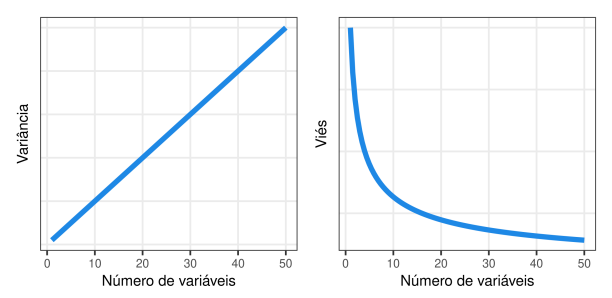
\includegraphics[width=0.9\linewidth]{vies_variancia.png}}
\caption{Comportamento assintótico do viés e da variância em função do número de covariáveis incluídas no modelo preditivo \cite{izbicki2020}.}
\label{fig:vies_variancia}
\end{figure}

Para alcançar o ponto de equilíbrio ótimo entre viés e variância (Figura \ref{fig:vies_variancia}), a prática habitual de aprendizado de máquina emprega validação cruzada $K$-Fold convencional. Todavia, em bases de dados forenses com ordenamento cronológico natural, o particionamento aleatório uniforme com embaralhamento (\textit{shuffling}) introduz severo vazamento de informação do futuro para o passado (\textit{look-ahead bias}), violando os pressupostos de causalidade temporal \cite{hyndman2021}.

Para contornar essa limitação e garantir integridade metodológica ao estudo, empregou-se a Validação Cruzada Temporal por Janela Expansiva (\textit{Time Series Split / Rolling Forecasting Origin}), preconizada por Hyndman e Athanasopoulos \cite{hyndman2021}. Nesse esquema, os dados são particionados em ordem estritamente cronológica: a cada dobra $k$, o treinamento restringe-se às safras processuais passadas $[0, t_k]$ e a validação ocorre unicamente sobre a janela temporal imediatamente subsequente $(t_k, t_{k+1}]$, simulando realisticamente o comportamento de um sistema preditivo em produção nos tribunais.

\subsection{Regressão Logística Penalizada}
Para estabelecer a linha de base (\textit{baseline}) interpretável do estudo, adotou-se a Regressão Logística. Em problemas de classificação binária nos quais a variável resposta assume desfechos de mérito $Y \in \{0, 1\}$, o modelo estima a probabilidade a posteriori condicionada ao vetor de atributos $\mathbf{x} \in \mathbb{R}^d$ por meio da função logística (sigmoide) \cite{izbicki2020}:
\begin{equation}
P(Y=1 \mid \mathbf{x}) = \frac{1}{1 + e^{-(\beta_0 + \mathbf{x}^T \boldsymbol{\beta})}}
\label{eq:logistic}
\end{equation}
onde $\beta_0$ representa o intercepto e $\boldsymbol{\beta}$ denota o vetor de coeficientes associados às covariáveis forenses padronizadas. A principal vantagem teórica da Regressão Logística reside em sua interpretabilidade direta: a transformação logit expressa linearmente o logaritmo da razão de chances (\textit{log-odds}), permitindo mensurar a força e a direção do impacto de cada órgão julgador e tema jurídico sobre a probabilidade de procedência.

Contudo, diante de matrizes de alta dimensionalidade geradas pela expansão de variáveis categóricas e assuntos da TPU, a estimação irrestrita conduz à instabilidade numérica por colinearidade e ao sobreajuste. Para mitigar a variância do estimador, introduz-se uma regularização penalizada sobre a magnitude dos coeficientes. Enquanto a penalização \textit{Ridge} ($L_2$) encolhe suavemente os coeficientes correlacionados sem anulá-los, a penalização \textit{Lasso} ($L_1$) força coeficientes irrelevantes exatamente a zero, operando seleção automática de atributos \cite{tibshirani1996, izbicki2020}.

Para usufruir simultaneamente de ambas as propriedades, implementou-se a regularização \textit{ElasticNet} \cite{zou2005}, cuja função de perda minimiza a log-verossimilhança negativa sob uma combinação convexa das normas $L_1$ e $L_2$:
\begin{equation}
\min_{\beta_0, \boldsymbol{\beta}} \left\{ -\frac{1}{N} \sum_{i=1}^N \Big[ y_i \ln(p_i) + (1 - y_i) \ln(1 - p_i) \Big] + \lambda \, \mathcal{P}_\alpha(\boldsymbol{\beta}) \right\}
\label{eq:elasticnet}
\end{equation}
onde $p_i = P(Y_i=1 \mid \mathbf{x}_i)$, $\lambda > 0$ é o coeficiente de regularização e o termo de penalidade mista é dado por \cite{zou2005}:
\begin{equation}
\mathcal{P}_\alpha(\boldsymbol{\beta}) = \alpha \|\boldsymbol{\beta}\|_1 + \frac{1 - \alpha}{2} \|\boldsymbol{\beta}\|_2^2 = \alpha \sum_{j=1}^d |\beta_j| + \frac{1 - \alpha}{2} \sum_{j=1}^d \beta_j^2
\label{eq:penalty_mix}
\end{equation}
onde $\alpha \in [0, 1]$ corresponde à proporção de mistura (\textit{l1\_ratio}). Na parametrização da biblioteca \textit{scikit-learn} \cite{pedregosa2011}, a intensidade global da penalidade é controlada inversamente por $C \propto 1/\lambda$, de modo que valores reduzidos de $C$ exercem maior contração sobre os parâmetros, promovendo estabilidade numérica e parcimônia.

\subsection{Métodos de Ensemble: Bagging e Boosting}
Para capturar potenciais interações não lineares entre o órgão julgador e a matéria processual, avaliaram-se métodos de comitê (\textit{ensembles}) baseados em Árvores de Decisão (CART) \cite{izbicki2020}. Uma árvore individual particiona o espaço de covariáveis em regiões hiper-retangulares disjuntas através de divisões binárias sucessivas (Figura~\ref{fig:arvore}). Em cada nó de partição $t$, a impureza de classificação binária é quantificada pelo Índice de Gini:
\begin{equation}
I_G(t) = 1 - \sum_{k=0}^1 p(k \mid t)^2 = 2\,p(1 \mid t)\,\big(1 - p(1 \mid t)\big)
\label{eq:gini}
\end{equation}
onde $p(k \mid t)$ representa a frequência relativa da classe $k$ no nó $t$. Embora apresentem baixo viés e capturem interações de alta ordem, árvores individuais padecem de elevada variância amostral frente a pequenas perturbações no conjunto de dados forenses \cite{izbicki2020}.

\begin{figure}[H]
\centering
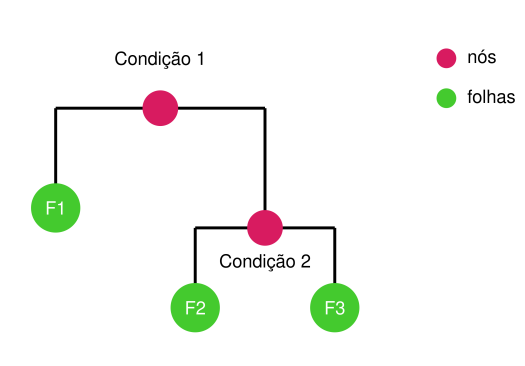
\includegraphics[width=0.78\linewidth]{arvore.png}
\caption{Exemplo da estrutura recursiva de uma árvore de decisão \cite{izbicki2020}.}
\label{fig:arvore}
\end{figure}

Para superar a fragilidade das árvores isoladas, adotou-se no Fluxo Alternativo 1 (FA1) a arquitetura de \textit{Random Forest} \cite{breiman2001}. O algoritmo ancora-se no princípio do \textit{Bagging} (\textit{Bootstrap Aggregating}), construindo um conjunto de $B$ árvores profundas descorrelacionadas, treinadas sobre réplicas amostrais geradas com reposição. A estimativa probabilística final do comitê é obtida pela média das predições individuais:
\begin{equation}
\hat{P}_{RF}(Y=1 \mid \mathbf{x}) = \frac{1}{B} \sum_{b=1}^B \hat{f}_b(\mathbf{x})
\label{eq:rf_prob}
\end{equation}
Para descorrelacionar os estimadores $\hat{f}_b$, o algoritmo restringe os atributos candidatos em cada nó a um subconjunto aleatório de tamanho $m \approx \sqrt{d}$, reduzindo substancialmente a variância do estimador combinado sem inflacionar o viés global \cite{breiman2001, izbicki2020}.

Em contrapartida, investigou-se no Fluxo Alternativo 2 (FA2) o algoritmo de gradiente impulsionado \textit{XGBoost} \cite{chen2016}. Diferente do aprendizado paralelo e independente da \textit{Random Forest}, o \textit{Boosting} opera via otimização sequencial aditiva de árvores rasas (\textit{weak learners}). Na $t$-ésima iteração aditiva, ajusta-se uma nova função $f_t$ para minimizar uma função objetivo penalizada:
\begin{equation}
\mathcal{L}^{(t)} = \sum_{i=1}^N l\left(y_i, \hat{y}_i^{(t-1)} + f_t(\mathbf{x}_i)\right) + \Omega(f_t)
\label{eq:xgboost_obj}
\end{equation}
onde $l$ denota a função de perda logarítmica (\textit{log-loss}) e $\Omega(f_t)$ penaliza explicitamente a complexidade da árvore através do número de folhas $T$ e do vetor de pesos das folhas $\mathbf{w} \in \mathbb{R}^T$ \cite{chen2016}:
\begin{equation}
\Omega(f_t) = \gamma T + \frac{1}{2}\lambda \sum_{j=1}^T w_j^2
\label{eq:xgboost_omega}
\end{equation}
onde $\gamma$ penaliza a criação de novas folhas e $\lambda$ controla a magnitude dos pesos dos nós terminais via regularização $L_2$, prevenindo sobreajustes e conferindo rigidez ao aprendizado sequencial.

\newpage
% --- V. METODOLOGIA ---
\section{Metodologia}

\subsection{Base de Dados e Particionamento Temporal}

\subsection{Engenharia de Atributos}

\subsection{Modelagem e Ajuste de Hiperparâmetros}

\subsection{Protocolo de Avaliação}

% --- VI. RESULTADOS E DISCUSSÃO ---
\section{Resultados e Discussão}

\subsection{Desempenho Comparativo no Teste Cego}

\subsection{Interpretabilidade e Análise dos Coeficientes}

% --- VII. CONCLUSÃO E TRABALHOS FUTUROS ---
\section{Conclusão e Trabalhos Futuros}

% --- REFERÊNCIAS BIBLIOGRÁFICAS (ORDENADAS ESTRITAMENTE POR ORDEM DE APARIÇÃO) ---
\begin{thebibliography}{99}

\bibitem{cnj_datajud}
Conselho Nacional de Justiça (CNJ), ``Resolução nº 331, de 20 de agosto de 2020: Institui a Base Nacional de Dados do Poder Judiciário -- DataJud,'' Brasília, DF, Brasil, 2020. [Online]. Available: \url{https://atos.cnj.jus.br/atos/detalhar/3428}

\bibitem{lage2022}
A.~Lage-Freitas, H.~Allende-Cid, O.~Santana, and L.~Oliveira-Lage, ``Predicting Brazilian court decisions,'' \emph{PeerJ Comput. Sci.}, vol.~8, Mar. 2022, Art. no.~e904, doi: 10.7717/peerj-cs.904.

\bibitem{bertalan2020}
V.~G.~F.~Bertalan and E.~E.~S.~Ruiz, ``Predicting judicial outcomes in the Brazilian legal system using textual features,'' in \emph{Proc. Workshop Digit. Humanities Nat. Lang. Process. (DHandNLP)}, Évora, Portugal, 2020, pp.~22--32. [Online]. Available: \url{http://ceur-ws.org/Vol-2607/paper3.pdf}

\bibitem{zabala2014}
F.~J. Zabala and F.~F. Silveira, ``Jurimetria: estatística aplicada ao direito,'' \emph{Rev. Direito e Liberdade}, vol.~16, no.~1, pp.~87--103, Jan./Apr. 2014. [Online]. Available: \url{https://ww2.esmarn.tjrn.jus.br/revistas/index.php/revista_direito_e_liberdade/article/view/732}

\bibitem{aletras2016}
N.~Aletras, D.~Tsarapatsanis, D.~Preo{\c{t}}iuc-Pietro, and V.~Lampos, ``Predicting judicial decisions of the European Court of Human Rights: A natural language processing perspective,'' \emph{PeerJ Comput. Sci.}, vol.~2, Oct. 2016, Art. no.~e93, doi: 10.7717/peerj-cs.93.

\bibitem{katz2017}
D.~M.~Katz, M.~J.~Bommarito~II, and J.~Blackman, ``A general approach for predicting the behavior of the Supreme Court of the United States,'' \emph{PLOS ONE}, vol.~12, no.~4, Apr. 2017, Art. no.~e0174698, doi: 10.1371/journal.pone.0174698.

\bibitem{izbicki2020}
R.~Izbicki and T.~M. dos Santos, \emph{Aprendizado de Máquina: Uma Abordagem Estatística}, 1st~ed. São Carlos, Brazil: Edição dos Autores, 2020.

\bibitem{priest1984}
G.~L. Priest and B.~Klein, ``The selection of disputes for litigation,'' \emph{J. Legal Stud.}, vol.~13, no.~1, pp.~1--55, Jan. 1984, doi: 10.1086/467732.

\bibitem{trecenti2021}
J.~A.~Z.~Trecenti, ``Diagramas de influência: uma aplicação em Jurimetria,'' M.S. thesis, Inst. Mat. Estat., Univ. São Paulo, São Paulo, Brazil, 2016, doi: 10.11606/D.45.2016.tde-20230727-113325.

\bibitem{hyndman2021}
R.~J. Hyndman and G.~Athanasopoulos, \emph{Forecasting: Principles and Practice}, 2nd~ed. Melbourne, Australia: OTexts, 2018.

\bibitem{miccibarreca2001}
D.~Micci-Barreca, ``A preprocessing scheme for high-cardinality categorical attributes in classification and prediction problems,'' \emph{ACM SIGKDD Explor. Newslett.}, vol.~3, no.~1, pp.~27--32, Jul. 2001, doi: 10.1145/507533.507538.

\bibitem{zou2005}
H.~Zou and T.~Hastie, ``Regularization and variable selection via the elastic net,'' \emph{J. Roy. Statist. Soc. Ser. B (Statist. Methodol.)}, vol.~67, no.~2, pp.~301--320, Apr. 2005, doi: 10.1111/j.1467-9868.2005.00503.x.

\bibitem{breiman2001}
L.~Breiman, ``Random forests,'' \emph{Mach. Learn.}, vol.~45, no.~1, pp.~5--32, Oct. 2001, doi: 10.1023/A:1010933404324.

\bibitem{chen2016}
T.~Chen and C.~Guestrin, ``XGBoost: A scalable tree boosting system,'' in \emph{Proc. 22nd ACM SIGKDD Int. Conf. Knowl. Discovery Data Mining}, San Francisco, CA, USA, 2016, pp.~785--794, doi: 10.1145/2939672.2939785.

\bibitem{pedregosa2011}
F.~Pedregosa et~al., ``Scikit-learn: Machine learning in Python,'' \emph{J. Mach. Learn. Res.}, vol.~12, pp.~2825--2830, Nov. 2011. [Online]. Available: \url{https://www.jmlr.org/papers/v12/pedregosa11a.html}

\bibitem{tibshirani1996}
R.~Tibshirani, ``Regression shrinkage and selection via the lasso,'' \emph{J. Roy. Statist. Soc. Ser. B (Methodol.)}, vol.~58, no.~1, pp.~267--288, 1996, doi: 10.1111/j.2517-6161.1996.tb02080.x.

\end{thebibliography}

\end{document}
